\section{Sistema de autenticación}

La protección del sistema y de los datos es algo fundamental en este proyecto. Cada usuario debe tener acceso a distintos recursos en base a su rol y se debe garantizar que un agente no registrado no pueda acceder al sistema. Para esto, se ha utilizado un sistema de autenticación basado en tokens. Esta era una alternativa que no dependía de otros servicios de autenticación externos y era lo suficientemente extendida para proporcionar una correcta seguridad al sistema. Junto con esto, esta alternativa es una de las más estandarizadas en la protección de APIs.

El funcionamiento es básico. Al usuario se le proporciona un token, firmado por una clave secreta en el proceso de login (representado en la Figura \ref{fig:ds-login}). A esta clave solo tendrá acceso el proceso correspondiente del servidor. Este token tendrá información cifrada acerca de la sesión, lo que permitirá que al realizar la autorización de acceso, no se tenga que validar la información del usuario accediendo a la base de datos, cosa que ralentizaría bastante el tiempo de respuesta del servidor. El usuario con este token podrá realizar peticiones, dentro de sus permisos. El funcionamiento de la autorización se explica esquemáticamente en el diagrama de secuencia de la Figura \ref{fig:ds-auth}.

\begin{figure}[]
    \centering
    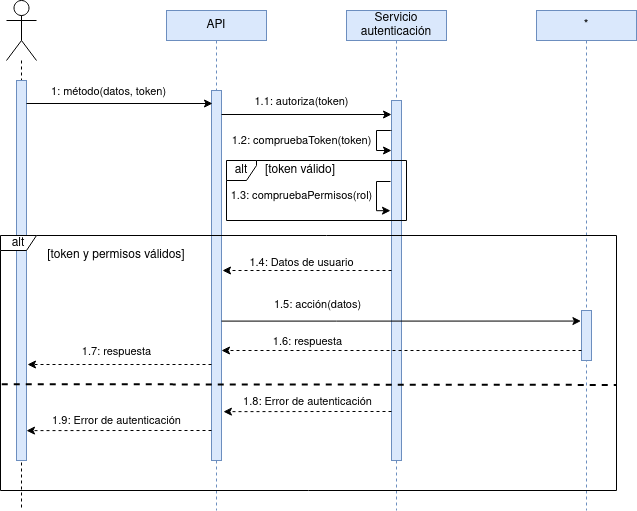
\includegraphics[width=\textwidth]{diseno/sistema/DS/autorizacion.png}
    \caption{Autorización del sistema}
    \label{fig:ds-auth}
\end{figure}

\begin{figure}[]
    \centering
    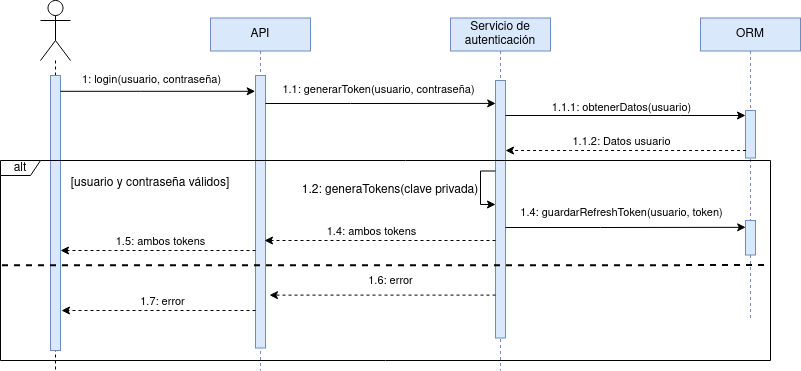
\includegraphics[width=\textwidth]{diseno/sistema/DS/login.png}
    \caption{Inicio de sesión en el sistema}
    \label{fig:ds-login}
\end{figure}

El token de autorización tiene una ``caducidad'' de 15 minutos. Esto será necesario debido a que, si el token no tuviese caducidad, un usuario eliminado o con los permisos modificados, podría seguir accediendo a zonas no autorizadas. Este tiempo ha sido elegido en base al tiempo de uso estimado por sesión. 

Para evitar que el usuario tenga que introducir su usuario y contraseña cada 15 minutos, se utiliza otro tipo de token. Este token será igual que el de autorización pero con la principal diferencia de que no caducará. Su utilidad será la de generar un nuevo token de autorización. Al generar un nuevo token de autorización, se comprobará la información del usuario en la base de datos, para proporcionar información de sesión actualizada en el nuevo token de autorización. El funcionamiento del token de refresh está esquemáticamente explicado en el diagrama de secuencia de la Figura \ref{fig:ds-refresh}.

\begin{figure}[]
    \centering
    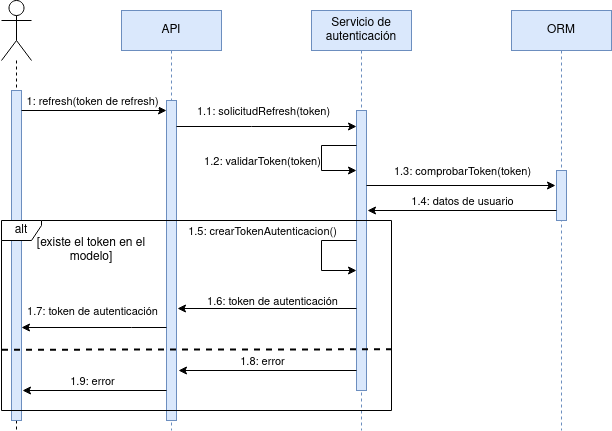
\includegraphics[width=\textwidth]{diseno/sistema/DS/refresh.png}
    \caption{Funcionamiento del token de refresh}
    \label{fig:ds-refresh}
\end{figure}

Los tokens de refresh válidos hasta el momento se almacenarán en la base de datos. Esto será así para que el usuario pueda invalidar los tokens mediante un cierre de sesión. El proceso de ``logout'' es el mostrado en la Figura \ref{fig:ds-logout}.   

\begin{figure}[]
    \centering
    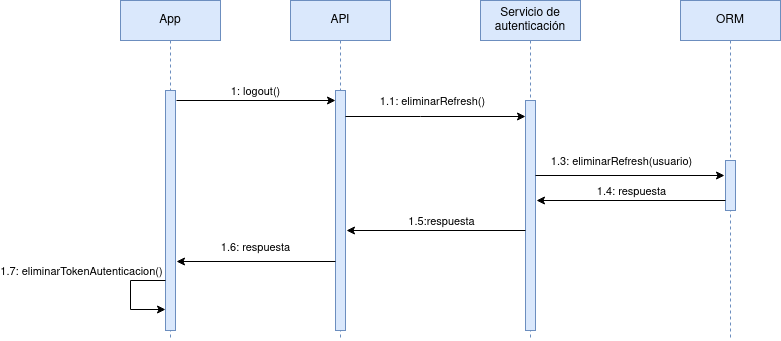
\includegraphics[width=\textwidth]{diseno/sistema/DS/logout.png}
    \caption{Cierre de sesión en el sistema}
    \label{fig:ds-logout}
\end{figure}

Todo esto permitirá controlar los usuarios actualmente logueados en el sistema, así como borrar usuarios, prohibiendo su acceso al eliminar su información del sistema, así como su token de refresh. Al editar un usuario, también garantizamos que como mucho, en los próximos 15 minutos estos cambios sean efectivos.

Todo el mecanismo de autorización se ha implementado con el objetivo de controlar correctamente los permisos de acceso de los usuarios, sin ver el rendimiento y el tiempo de respuesta del servidor afectado. 